\subparagraph{Periodic Term} \label{Periodic Term}
The terms discussed so far have been mathematically quite simple, though that is not the case for the periodic term. Unlike the other terms, each element consists of an infinite sum. This would suggest that simplifications might be necessary, but it is clear that the largest number possible of significant figures has been used so far \textendash\ this has been the case due to the periodic term, which as will discussed below, requires as many significant figures as possible in order to provide appropriate results (Miroshnychenko, Y., personal communication, October 2017).

For our calculations, we will be utilising $\rho$ with an accuracy of 9 significant figures, though for the sake of brevity the data displayed will be far more concise. The first value of $\rho$ is $\frac{1}{2} + i14.134725$ \citep{UMNZetaZeros}, so for $100^\rho$:

\begin{equation}
\begin{split}
	100^{\rho} &=100^{\frac{1}{2} + 14.134725i} = 100^{\frac{1}{2}} \cdot 100^{14.134725i} = 10 \cdot e^{\ln 100^{14.134725i}}\\
		&= 10 \cdot e^{4.605170 \cdot 14.134725i} = 10 \cdot e^{65.092812i} = 10 \cdot e^{10.359842\cdot 2\pi i} \\
		&= 10 \cdot \cancelto{1}{e^{10 \cdot 2\pi i}} \cdot e^{0.359842 \cdot 2\pi i} \\
		& \therefore 100^{\rho} = 10 \cdot e^{2.260954i}\\
\end{split}
\end{equation}

This is compared to the calculation for $\rho_t = \frac{1}{2} + i14$:
\begin{equation}
\begin{split}
	100^{\rho_t} &= 100^{\frac{1}{2}} \cdot e^{4.605170 \cdot 14i} = 10 \cdot e^{64.472380i} \\
				&= 10 \cdot \cancelto{1}{e^{10\cdot 2\pi i}} \cdot e^{0.261098 \cdot 2\pi i}\\
				&\therefore 100^{\rho_t} = 10 \cdot e^{1.640527i}
\end{split}
\end{equation}

By plotting both $100^{\rho}$ and $100^{\rho_t}$ into an Argand diagram, as can be seen in figure \ref{gr:ArgandSimplificationOfRho}. Finally, figure \ref{gr:ArgrandOfLiRho} makes it really clear that simplifications will indeed lead to a very large change in value for the periodic term.
\begin{figure}[h]
\begin{subfigure}{.5\textwidth}
	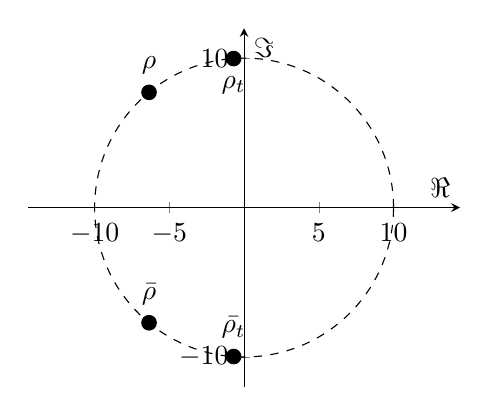
\begin{tikzpicture}
	\begin{axis}[
	scale=0.8,
	xmin=-12, xmax = 12,
	ymin=-12, ymax=12,
	axis equal, axis lines = center,
	xlabel=$\mathbb{\Re}$, ylabel=$\mathbb{\Im}$
	]
	
	\node [circle, fill, inner sep=2pt, label={$\rho$}]
		at (axis cs: -6.36,7.71){};
	\node [circle, fill, inner sep=2pt, label={$\bar{\rho}$}] %conjugate
		at (axis cs: -6.36,-7.71){};
		
	\node [circle, fill, inner sep=2pt, label={below:$\rho_t$}]
		at (axis cs: -0.70,9.97){};
	\node [circle, fill, inner sep=2pt, label={$\bar{\rho_t}$}] %conjugate
		at (axis cs: -0.70,-9.97){};
		
	\draw [dashed, black] (axis cs: 0, 0) circle [radius=10];
	\end{axis}
	\end{tikzpicture}
	\caption{Argand diagram of $\rho = \frac{1}{2} + 14.134725i$, \\ $\rho_t = \frac{1}{2} + 14i$ and their respective conjugates}
	\label{gr:ArgandSimplificationOfRho}
\end{subfigure}%
\begin{subfigure}{.45\textwidth}
	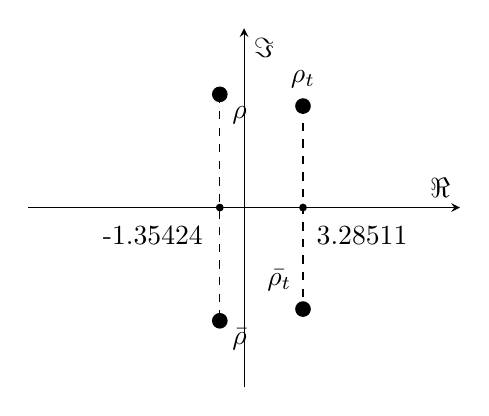
\begin{tikzpicture}
	\begin{axis}[
	scale=0.8,
	xlabel=$\mathbb{\Re}$, ylabel=$\mathbb{\Im}$,
	ticks = none, axis equal, axis lines = center,
	xmin=-10, xmax = 10, ymin=-10, ymax=10,
	]
	
	\node [circle, fill, inner sep=2pt, label={[xshift=0.25cm, yshift=-0.6cm] $\rho$}]
		at (axis cs: -1.35424,6.31435){};
	\node [circle, fill, inner sep=2pt, label={[xshift=0.25cm, yshift=-0.6cm] $\bar{\rho}$}]
		at (axis cs: -1.35424,-6.31435){}; %conjugate
	\draw [dashed] (axis cs:-1.35424,6.31435) -- (axis cs:-1.35424,-6.31435);
	\node [circle, fill, inner sep = 1pt, label = {[xshift=-0.85cm,yshift=-0.65cm]-1.35424}]
		at (axis cs:-1.35424, 0){};
	
	\node [circle, fill, inner sep=2pt, label={$\rho_t$}]
		at (axis cs: 3.28511,5.66089){};
	\node [circle, fill, inner sep=2pt, label={[xshift=-0.3cm]$\bar{\rho_t}$}] 
		at (axis cs: 3.28511,-5.66089){}; %conjugate
	\draw [dashed] (axis cs:3.28511,5.66089) -- (axis cs:3.28511,-5.66089);
	\node [circle, fill, inner sep = 1pt, label = {[xshift=0.75cm,yshift=-0.65cm]3.28511}]
		at (axis cs:3.28511,0){};
	\end{axis}
	\end{tikzpicture}
	\caption{Argand diagram of $li(\rho)$ and $li(\rho_t)$, and respective conjugates}
	\label{gr:ArgrandOfLiRho}
\end{subfigure}
\end{figure}

\subparagraph{Calculations} Despite the need for infinitely many terms, for the sake of demonstration we will take only the first forty zeros \citep{UMNZetaZeros} and their conjugates for the first element of the periodic term. The calculations are done through Mathematica.
\begin{equation}
\begin{split}
	&1a: li(100^{\frac{1}{2}+i14.134725}) = li(-6.36664 + i7.71141) = 1.35421 + i6.31436\\
	&1b: li(100^{\frac{1}{2}-i14.134725}) = li(-6.36664 - i7.71141)= 1.35421 - i6.31436\\
	&2a: li(100^{\frac{1}{2}+i21.022039}) = li(-8.36843 + i5.47442)= 0.452923 + i6.28610\\
	&2b: li(100^{\frac{1}{2}-i21.022039}) = li(-8.36843 - i5.47442) = 0.452923 - i6.28610\\
\end{split}
\end{equation}

The addition of the first forty zeros ($\rho$) for the very first term of the periodic term (that is, $li(n^{\rho}))$ and their respective conjugates can be seen in Appendix \ref{Data}, Table \ref{tb:LiValuesFor100}. Though what is important is that they add up to about 255. Thus, we use our known value of $\pi(100)$ from earlier sieving in order to verify whether our findings are logical. We do so by utilising equation \ref{eq:ExampleOfFinalPi(n)}.
\begin{equation*}
\begin{split}
	&\pi(100) = \text{Principal + Secondary + Integral + Log + Periodic} \\
	&25 = 30.1261416 - 4.34495202 - 0.000259962 - 0.092419624 + \text{ Periodic}\\
	&\text{Periodic} = -0.688509994
\end{split}
\end{equation*}
This means that somehow our calculations are completely nonsensical, as we are expecting the sum of all periodic terms to be -0.7 and the very first term is already 255! In attempting to uncover what is generating this error, we compare Derbyshire's provided example calculations for $li(20)$ \citep[p.340]{derbyshire2003prime} to our results with Mathematica (Appendix \ref{ap:MathematicaLi}), as seen below.
\begin{table}[h]
	\centering
\begin{tabular}{c|c|c}
										& Derbyshire 			& Mathematica \\ \hline
	$20^{(\frac{1}{2}+i14.134725)}$		& $-0.302303 - i4.46191$& $ -0.302305 - i4.46191 $\\
	$li(20^{(\frac{1}{2}+i14.134725)})$	& $-0.105384 - i3.14749$& $ 0.952805 - i3.91384 $\\
\end{tabular}
\caption{Comparison of known values \citep[p.340]{derbyshire2003prime} for complex exponentiation and logarithmic integral. (Mathematica, Appendix \protect\ref{ap:MathematicaLi})}
\end{table}

So why is this happening? In solving $\ln(n^{\rho})$, Mathematica is not returning $\rho \ln n$, but rather $\rho \ln n - 2k\pi i$ where $k$ is a value such that the imaginary part of the solution lie between $-\pi$ and $\pi$ \citep[p.548]{wagon1999mathematica}, leading to the incorrect sum we are observing. As this is a quirk of the software, we won't be discussing it in great deal, but the solution, according to Wagon, lies in utilising the Exponential Integral function, $Ei(n)$, whose relationship with $li(n)$ is as follows.
\begin{equation*}
	li(n^{\rho}) = Ei( \ln n^{\rho} )
\end{equation*}

We repeat the calculations in Mathematica utilising $Ei(n)$ (Algorithm: Appendix \ref{ap:MathematicaEi}), add each respective conjugate like done previously (Appendix \ref{Data}, table \ref{tb:EiValuesFor100}). The process is then done for the entire periodic term, as per the algorithm in Appendix \ref{ap:MathematicaSumOfEi}, which yields the value of $-0.573055632$. Incredibly close to the expected $-0.688509994$, especially since we only used forty terms! Thus, we can affirm the value of $\pi(100)$, and have shown that equation \ref{eq:pi(n)fromJ(n)} can indeed tell us how many primes there are between 1 and $n$.
\begin{equation*}
\begin{split}
	&\pi(100) = 30.1261416 - 4.34495202 -0.573055632 - 0.000259962 - 0.092419624\\
	&\therefore  \pi(100) = 25
\end{split}
\end{equation*}